\titledquestion{Disjoint Set Practice}

Given the following set of operations on a disjoint set(initially there are six disjoint elements), show the final disjoint set tree for each of the following optimization strategies:

\begin{itemize}
    \item $set\_union(A, B)$
    \item $set\_union(C, D)$
    \item $set\_union(B, C)$
    \item $find(D)$
    \item $set\_union(E, F)$
    \item $set\_union(E, A)$
\end{itemize}

\begin{parts}
    \part[5] Only with union-by-rank optimization. (When two trees have the same height, the set specified first in the union will be the root of the merged set.)
    \begin{solution}
        \begin{center}
            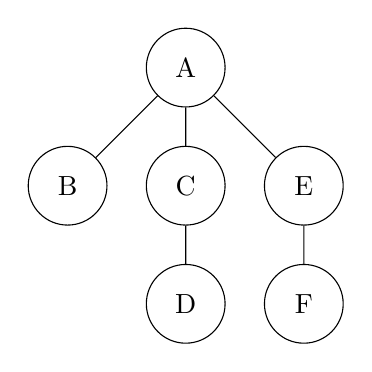
\begin{tikzpicture}[
                every node/.style={circle, draw, minimum size=1cm, inner sep=0pt},
                level 1/.style={sibling distance=15mm},
                edge to parent/.style={draw, -latex}
            ]
            
            % Root node
            \node {A}
                child {node {B}}
                child {node {C} child{node{D} } }
                child {node {E} child{node{F} } };
            
            \end{tikzpicture}
        \end{center}
    \end{solution}
    \part[5] Only with path compression. (The set specified first in the union will always be the root of the merged set.)
    \begin{solution}
        \begin{center}
            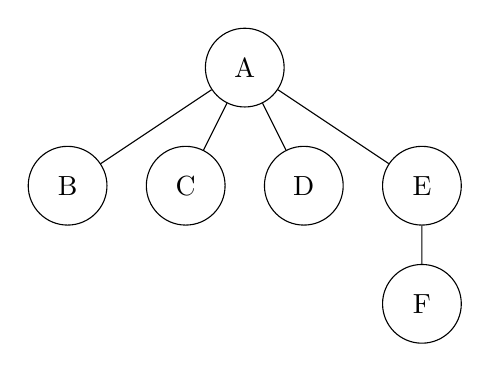
\begin{tikzpicture}[
                every node/.style={circle, draw, minimum size=1cm, inner sep=0pt},
                level 1/.style={sibling distance=15mm},
                edge to parent/.style={draw, -latex}
            ]
            
            \node {A}
                child {node {B}}
                child {node {C}}
                child {node {D}}
                child {node {E} child{node{F} } };
            
            \end{tikzpicture}
        \end{center}
    \end{solution}
\end{parts}
